\documentclass[12pt]{article}

% ── Packages ──────────────────────────────────────────────────────────────────
\usepackage[margin=1in]{geometry}
\usepackage{booktabs}
\usepackage{amsmath, amssymb}
\usepackage{graphicx}
\usepackage{subcaption}
\usepackage{hyperref}
\usepackage{microtype}
\usepackage{parskip}
\usepackage{xcolor}
\usepackage{enumitem}
\usepackage{tabularx}
\usepackage{natbib}
\usepackage{setspace}

\hypersetup{colorlinks=true, linkcolor=blue, citecolor=blue, urlcolor=blue}
\graphicspath{{figures/}}

% ── Metadata ──────────────────────────────────────────────────────────────────
\title{Zeitgeist Machine:\\
       Activation Geometry Tracks Survey Polarization}
\author{}
\date{\today}

% ══════════════════════════════════════════════════════════════════════════════
\begin{document}
\maketitle

\begin{abstract}
    TODO
\end{abstract}

\tableofcontents
\newpage

% ── Sections ──────────────────────────────────────────────────────────────────
\section{Introduction}
\label{sec:intro}

TODO
1. Conceptual graph of the four quadrants.


2. Rhetorical vs. stance, Politician (elite) vs Mass


3. LLM vs  opinion survey vs voting behavior


4. Mismatch: a. political rhetorical false polarization

\section{Methodology}
\label{sec:methods}

% ── Overview ──────────────────────────────────────────────────────────────────
\subsection{Overview}

We ask whether the partisan geometry encoded in LLM attention activations tracks real issue partisanship as measured by survey responses. For each of $T$ political topics, we compute two quantities:
\begin{enumerate}
    \item \textbf{Activation-space partisan divergence}: the Mahalanobis distance between Democrat and Republican centroids in a per-head PCA-reduced activation space.
    \item \textbf{Survey partisanship}: the normalized partisan gap in GSS response means.
\end{enumerate}
The main outcome is the Pearson $r$ (and Spearman $\rho$) between these two vectors across all $T$ topics.

% ── GSS ───────────────────────────────────────────────────────────────────────
\subsection{Survey Partisanship Measure}
\label{sec:gss}

For each topic $t$, we compute the survey-measured partisan gap from the General Social Survey (GSS) 2021--2024 cumulative dataset:
\begin{equation}
    \delta_t = \frac{|\bar{x}^R_t - \bar{x}^D_t|}{s_t}
    \label{eq:gss_pol}
\end{equation}
where $\bar{x}^D_t$ and $\bar{x}^R_t$ are the mean response codes among Democrats and Republicans respectively, and $s_t$ is the range of the response scale (i.e., the maximum minus the minimum response code), normalizing $\delta_t \in [0,1]$ regardless of the original scale. Topics are included only if at least 100 Democrats and 100 Republicans responded ($n_D \geq 100$, $n_R \geq 100$, $n \geq 200$ total).

\paragraph{Party coding.}
Respondents are classified by the GSS \texttt{partyid} variable on a 7-point scale:
\begin{center}
\begin{tabular}{clc}
\toprule
\texttt{partyid} & Label & Party \\
\midrule
0 & Strong Democrat           & $D$ \\
1 & Not strong Democrat       & $D$ \\
2 & Independent, near Dem.    & $D$ \\
3 & Independent               & \textit{excluded} \\
4 & Independent, near Rep.    & $R$ \\
5 & Not strong Republican     & $R$ \\
6 & Strong Republican         & $R$ \\
\bottomrule
\end{tabular}
\end{center}

\paragraph{Topic scope.}
We analyze two categories of GSS topics:
\begin{itemize}
    \item \textbf{Public issues} ($T_\text{pub} = 126$): questions about policy, government, and social issues. Eight topics are excluded whose wording contains explicit racial comparison framing that would conflate attitude with world knowledge (\texttt{hubbywk1}, \texttt{racdif1}--\texttt{racdif4}, \texttt{workwhts}, \texttt{wlthwhts}, \texttt{intlwhts}).
    \item \textbf{Private life} ($T_\text{priv} = 73$): questions about personal behavior, religious practice, and lifestyle (e.g., church attendance, sexual attitudes, family structure). Five topics are excluded due to ambiguous framing (\texttt{reborn}, \texttt{marwht}, \texttt{helpful}, \texttt{helpfulnv}, \texttt{helpfulv}).
\end{itemize}

% ── Activation extraction ─────────────────────────────────────────────────────
\subsection{Activation Extraction}
\label{sec:extraction}

We register forward hooks on the output-projection layer (\texttt{o\_proj}) of each of the $L$ transformer layers, capturing \texttt{input[0]} — the pre-projection concatenated head outputs — of shape $[B, S, H{\cdot}D_h]$. This is reshaped to $[B, S, H, D_h]$ and the \textbf{last token position} $[:,{-1},:,:]$ is retained, yielding shape $[B, H, D_h]$.

Capturing the \emph{input} to \texttt{o\_proj} (rather than the output) allows clean decomposition into individual heads, since the projection mixes heads after this point. After all $N$ prompts are processed in batches, activations are concatenated to $\mathbf{X} \in \mathbb{R}^{N \times L \times H \times D_h}$.

% ── PCA Mahalanobis ───────────────────────────────────────────────────────────
\subsection{Per-Head Mahalanobis Distance}
\label{sec:mahal}

For each attention head $(l, h)$, extract $\mathbf{X}_{lh} = \mathbf{X}[:, l, h, :] \in \mathbb{R}^{N \times D_h}$ (typically $D_h = 128$) and proceed as follows:

\begin{enumerate}[label=\arabic*.]
    \item \textbf{PCA}: Fit on all $N$ rows pooled and reduce to $k = \min(15, D_h, N{-}1)$ components, giving $\tilde{\mathbf{X}}_{lh} \in \mathbb{R}^{N \times k}$.

    \item \textbf{Party centroids}: Partition rows into Democrats $\mathcal{D}$ and Republicans $\mathcal{R}$. The centroid for party $P \in \{D, R\}$ is the mean of its members' PCA-projected activations:
    \begin{equation}
        \boldsymbol{\mu}_P = \frac{1}{|\mathcal{P}|}\sum_{i \in \mathcal{P}} \tilde{\mathbf{x}}_i
        \label{eq:centroid}
    \end{equation}
    where $\tilde{\mathbf{x}}_i \in \mathbb{R}^k$ is the PCA-projected activation for subject $i$. As a robustness check, we can also do the coordinate-wise median for the centroid in place of $\boldsymbol{\mu}_P$.

    \item \textbf{Pooled covariance}:
    \begin{equation}
        \boldsymbol{\Sigma} = \tfrac{1}{2}(\boldsymbol{\Sigma}_D + \boldsymbol{\Sigma}_R) + \varepsilon\mathbf{I}, \quad \varepsilon = 10^{-6}
    \end{equation}

    \item \textbf{Mahalanobis distance}:
    \begin{equation}
        m_{lh} = \sqrt{(\boldsymbol{\mu}_D - \boldsymbol{\mu}_R)^\top \boldsymbol{\Sigma}^{-1} (\boldsymbol{\mu}_D - \boldsymbol{\mu}_R)}
        \label{eq:mahal}
    \end{equation}
\end{enumerate}

This is computed in parallel for each of the $L \times H$ heads, producing a grid $\mathbf{M} \in \mathbb{R}^{L \times H}$. Two summary statistics aggregate the grid:
\begin{align}
    m^\text{all} &= \frac{1}{LH}\sum_{l,h} m_{lh} \label{eq:mall} \\
    m^\text{mid} &= \text{mean}_{l \in \mathcal{L}_\text{mid},\, h}\; m_{lh} \label{eq:mmid}
\end{align}
where $\mathcal{L}_\text{mid} = \{l : \lfloor 0.45L \rfloor \le l < \max(\lfloor 0.55L \rfloor, \lfloor 0.45L \rfloor{+}1)\}$ selects the middle 10\% of layers. Empirically, $m^\text{mid}$ performs worse than $m^\text{all}$ for deep models ($L \ge 70$), with correlations reduced by up to 0.48.

% ── Simulation methods ────────────────────────────────────────────────────────
\subsection{Simulation Methods}
\label{sec:sim}

We test two methods for constructing the $N$ prompts per topic.

\subsubsection{Politician Simulation}
\label{sec:politician}

\paragraph{Subjects.} 550 members of the 116th U.S. Congress with valid name and party affiliation from the DW-NOMINATE dataset.

\paragraph{Prompt conditions.} One prompt is generated per politician per topic ($N = 550$). Each prompt is prefixed by a system message that frames the politician-simulation task. The system message was varied across nine phrasings to verify robustness; alignment differs by less than $0.025$ across all variants (Appendix~\ref{app:sys_msg}). Three user-turn conditions are tested:

\begin{center}
\small
\begin{tabular}{lp{5.5cm}p{5.5cm}}
\toprule
Condition & Instruct template & Base template \\
\midrule
\textsc{rhetorical} & \texttt{Generate a statement by \{name\} on \{topic\}.} & \texttt{\{name\} makes a statement on \{topic\}:} \\
\textsc{stance}     & \texttt{What is \{name\}'s position on \{topic\}?}     & \texttt{On \{topic\}, \{name\}'s position is} \\
\textsc{survey}     & \texttt{If asked in a national survey about \{topic\}, how would \{name\} respond?} & \texttt{In a survey about \{topic\}, \{name\} would respond} \\
\bottomrule
\end{tabular}
\end{center}

\texttt{\{topic\}} is a natural-language clause derived from the GSS question wording. Table~\ref{tab:topic_examples} lists representative topics from both categories. Public-issue topics cover policy and governance; private-life topics cover personal behaviour, moral attitudes, and lifestyle---areas where partisan sorting is less explicit in political discourse but nonetheless present in survey data.

\begin{table}[ht]
\centering
\small
\caption{Sample GSS topics and their natural-language clauses used in prompts.}
\label{tab:topic_examples}
\begin{tabular}{llp{8cm}}
\toprule
Variable & Category & Natural-language clause \\
\midrule
\texttt{abhelp2}  & public  & whether to help pay for an abortion \\
\texttt{gunlaw}   & public  & whether to favor or oppose requiring a permit to buy a gun \\
\texttt{eqwlth}   & public  & whether the government should reduce income differences between the rich and poor \\
\texttt{grass}    & public  & whether marijuana should be made legal \\
\texttt{confinan} & public  & the level of confidence in banks and financial institutions \\
\texttt{nextgen}  & public  & whether science and technology will give more opportunities to the next generation \\
\midrule
\texttt{spanking}  & private & whether it is sometimes necessary to discipline a child with spanking \\
\texttt{evstray}   & private & whether to have sex with someone other than a spouse while married \\
\texttt{marmakid}  & private & whether a single mother can raise a child as well as a married couple \\
\texttt{fear}      & private & whether to be afraid to walk alone at night in the neighborhood \\
\texttt{life}      & private & whether life is exciting, routine, or dull \\
\texttt{marasian}  & private & how to feel about a close relative marrying an Asian American person \\
\bottomrule
\end{tabular}
\end{table}

To illustrate the full prompts fed to the model, the following are concrete instantiations across prompt conditions and topics, each preceded by the system message \textit{``You are simulating the public stance of U.S.\ politicians.''}:

\begin{itemize}[leftmargin=*]
    \item \textsc{stance}, public topic: \textit{``What is Ted Cruz's position on whether to help pay for an abortion?''}
    \item \textsc{rhetorical}, public topic: \textit{``Generate a statement by Alexandria Ocasio-Cortez on the level of confidence in banks and financial institutions.''}
    \item \textsc{survey}, public topic: \textit{``If asked in a national survey about whether to favor or oppose requiring a permit to buy a gun, how would Mitt Romney respond?''}
    \item \textsc{stance}, public topic: \textit{``What is Elizabeth Warren's position on whether marijuana should be made legal?''}
    \item \textsc{survey}, private topic: \textit{``If asked in a national survey about whether to have sex with someone other than a spouse while married, how would Mitt Romney respond?''}
    \item \textsc{stance}, private topic: \textit{``What is Nancy Pelosi's position on whether it is sometimes necessary to discipline a child with spanking?''}
    \item \textsc{rhetorical}, private topic: \textit{``Generate a statement by Marsha Blackburn on whether a single mother can raise a child as well as a married couple.''}
    \item \textsc{survey}, private topic: \textit{``If asked in a national survey about whether life is exciting, routine, or dull, how would Marco Rubio respond?''}
\end{itemize}

The private-life examples highlight a distinctive feature of this study: models are asked to simulate politicians on topics---marital fidelity, parenting practices, neighbourhood safety---that rarely appear in legislative records or campaign rhetoric, yet still exhibit partisan structure in survey data.

The three conditions test distinct representational hypotheses: \textsc{rhetorical} tests whether political speech generation is organized by partisan identity; \textsc{stance} tests factual belief-attribution; \textsc{survey} tests whether the model tracks response-style differences between parties.

\subsubsection{Demographic Simulation}
\label{sec:demo}

\paragraph{Subjects.} For each topic $t$, we include all GSS 2021–2024 respondents who (a) provided a valid response to topic $t$ and (b) are classified as Democrat or Republican. We evaluate two sampling settings:
(1) a \textbf{stratified sampling} condition, in which a 10\% sample is drawn stratified on \texttt{polviews}, \texttt{age\_bin}, \texttt{degree}, \texttt{race}, \texttt{sex}, and \texttt{rincome}, requiring at least 10 respondents per party; and
(2) a \textbf{non-stratified} condition, where respondents are sampled without demographic stratification. This allows us to assess the impact of sampling design on simulation outcomes.

\paragraph{Persona profile.} Each respondent is represented by up to 83 demographic fields. For each non-missing field, numeric codes are mapped to human-readable strings using Stata value labels (e.g., \textit{`Age: 45''}, \textit{`Education: Bachelor’s degree''}). Fields are concatenated using ``\texttt{. }'' as a separator and \textbf{randomly shuffled per topic} (seeded by \texttt{hash(topic)}) to mitigate ordering artifacts.

In addition to the full-profile setting, we conduct a \textbf{focused demographic study} using a reduced profile containing only key attributes: \texttt{age}, \texttt{sex}, \texttt{race}, \texttt{relig}, and \texttt{occ}. This enables analysis of how model behavior changes when only core demographic signals are provided.

\paragraph{Prompt (Format B, default).}
\begin{quote}
\textit{System}: ``You are simulating the views of an American.''\\[2pt]
\textit{User}: ``Given the following background about a person:\\
\quad\texttt{\{profile\}}\\[2pt]
How would they answer: \texttt{\{survey\_question\}}''
\end{quote}

To prevent leakage, any lifestyle variable that coincides with the current survey topic is excluded from that respondent's profile for that topic.

% ── Alignment metric ──────────────────────────────────────────────────────────
\subsection{Alignment Metric}
\label{sec:alignment}

For a given simulation method, condition, and layer-selection variant, we correlate the vector of activation-space partisan divergence scores $\hat{\boldsymbol{\delta}}$ with the GSS partisanship vector $\boldsymbol{\delta}$ across all $T$ topics in the category ($T_\text{pub} = 126$ or $T_\text{priv} = 73$):
\begin{align}
    r &= \mathrm{Pearson}(\hat{\boldsymbol{\delta}},\, \boldsymbol{\delta}) \\
    \rho &= \mathrm{Spearman}(\hat{\boldsymbol{\delta}},\, \boldsymbol{\delta})
\end{align}

A high $r$ indicates that topics generating high partisan divergence in LLM activations are the same topics where actual survey respondents diverge most.

\paragraph{Politician vs.\ demographic comparison.}
When $r_\text{politician} > r_\text{demo}$, the model's parametric political knowledge (accessed via named politician prompts) more faithfully mirrors the GSS partisanship landscape than explicit demographic conditioning on real respondent data. This reflects a difference between what the model \emph{knows} about which topics are contested between parties and how it \emph{behaves} when role-playing constrained personas.

% ── Cultural Terrain Discovery ────────────────────────────────────────────────
\subsection{Cultural Terrain Discovery}
\label{sec:discovery}

The preceding analyses validate the activation-based partisan-divergence measure against known GSS topics. We additionally apply the same measure in an \emph{unsupervised discovery} mode: given a large corpus of novel opinion clauses not drawn from any existing survey instrument, which topics does the model flag as highly partisan in activation space? High-scoring topics from this scan are candidates for survey items that existing instruments do not cover.

\paragraph{Corpus construction.}
We assembled a corpus of approximately 1.3 million candidate clauses from four source collections (Table~\ref{tab:discovery_corpora}). Raw items from each source --- bill titles, academic abstracts, social-media posts, and encyclopaedic descriptions --- were converted into natural-language opinion clauses of the form ``the [noun phrase]'' or ``whether [subordinate clause]'', matching the format of GSS topic wording. Clause generation used an instruction-tuned model prompted to reframe each item as a topic on which people can hold opposing views; items that could not be meaningfully reformulated (purely factual content, data artefacts) were discarded.

\begin{table}[ht]
\centering
\small
\caption{Source corpora for cultural terrain discovery.}
\label{tab:discovery_corpora}
\begin{tabular}{lrp{7.5cm}}
\toprule
Source & Clauses & Content \\
\midrule
Merged (multi-source) & 477,343 & Wikipedia articles, Reddit opinion posts, news headlines, memes, party platforms, ballot measures, book and film titles, ATUS time-use labels \\
Congress bills        & 359,302 & U.S. Congress bill titles and CRS report summaries \\
Web of Science        & 424,445 & Academic abstract text, restricted to social-science and humanities journals \\
Reddit (partisan)     &  47,018 & Posts from politically-aligned subreddits, filtered to surface-apolitical wording \\
\midrule
Total                 & 1,308,108 & \\
\bottomrule
\end{tabular}
\end{table}

\paragraph{Scoring.}
Each clause is scored using the identical pipeline as Section~\ref{sec:mahal}: the same 550 Congress members, the same \textsc{stance} prompt template, the same \texttt{o\_proj} activation extraction, PCA reduction ($k = 15$), and mean Mahalanobis distance $m^\text{all}$ averaged across all $L \times H$ heads. The scoring model is dolphin-2.9.3-llama-3-8b (8B) with the roleplay system message (Appendix~\ref{app:sys_msg}). Because each clause is scored independently using the same partisan geometry that correlates $r \approx 0.74$ with GSS partisanship on known topics, the $m^\text{all}$ score serves as a proxy for expected survey-measured partisanship.

\paragraph{Output.}
The top-scoring clauses from each corpus are retained as candidate survey items. Table~\ref{tab:discovery_top} (Section~\ref{sec:results_discovery}) lists representative high-scoring examples. Because the scoring is unsupervised --- no ground-truth partisanship labels are used --- the discovered topics represent the model's implicit map of the partisan cultural terrain, extending well beyond the policy and lifestyle domains covered by the GSS.

\paragraph{Surprise analysis: latent partisan structure.}
A high $m^\text{all}$ score is not itself surprising if the clause is overtly political --- a bill about abortion policy or an article titled ``Republican efforts to restrict voting'' would be expected to produce partisan activation geometry. The more scientifically interesting case is a topic that is \emph{more} polarized than its surface content predicts. We isolate these cases via a two-stage regression procedure.

\textit{Stage 1 --- Political content scoring.} Each clause is embedded with a 300M-parameter Gemma3-backbone sentence encoder (mean-pooled, L2-normalised, 768-dimensional). The political content of a clause is operationalised as its cosine similarity to a set of 234 Ballotpedia ballot-measure subtopics spanning ten parent categories (Budget and Tax, Criminal Justice, Education, Elections, Environment, Governance, Infrastructure, Labour and Healthcare, Military, and Social Issues). These anchor similarities form a feature vector of political salience.

\textit{Stage 2 --- Per-corpus OLS and residual.} Within each corpus separately, we regress $m^\text{all}$ on the 234 anchor-similarity features using ordinary least squares with 5-fold cross-validation ($K = 5$). Fitting per-corpus rather than pooled avoids confounding the baseline polarization level across sources (congressional bill clauses are almost universally political; AITA interpersonal-dilemma posts are almost universally apolitical). The surprise score for clause $i$ in corpus $c$ is the OLS residual:
\begin{equation}
    s_i = m^\text{all}_i - \hat{m}^\text{all}_i
\end{equation}
where $\hat{m}^\text{all}_i$ is the within-corpus predicted value. A large positive residual indicates that the model's activation geometry flags the topic as politically contentious even though the clause's semantic content offers little indication of political relevance.

\textit{Non-political filter.} To surface genuinely surprising topics rather than noisily phrased political ones, we restrict attention to clauses whose predicted polarization $\hat{m}^\text{all}_i$ falls below the corpus mean. Within this filtered set, clauses are ranked by $s_i$ descending. We retain the top 1,000 per eligible corpus (AITA and Reddit; WoS, Wikipedia, and Congress are too uniformly political or too sparse after filtering).

\textit{Out-of-sample validation.} To test whether the surprise score generalises, we hand-curated 21 contemporary topics not drawn from any scraped corpus --- including items such as the tradwife lifestyle, raw milk consumption, fluoride removal from drinking water, and similar culturally-charged but explicitly non-partisan issues. We first predict their polarization using the per-corpus Ridge model, then measure actual $m^\text{all}$ scores using the dolphin-2.9.3-llama-3-8b pipeline, and compare predicted versus actual to confirm that the surprise decomposition transfers to genuinely novel clauses.

% ── Question Fundamentalness ──────────────────────────────────────────────────
\subsection{Question Fundamentalness (will elaborate later)}
\label{sec:fundamentalness}

A complementary analysis asks which survey topics are structurally \emph{central} to the opinion landscape --- topics whose activation geometry is most informative and whose responses are most predictive of others.

\paragraph{LLM-side measure.}
For each topic $t$, the per-head Mahalanobis scores $\{m_{lh}\}$ (Section~\ref{sec:mahal}) are aggregated into a single activation-based fundamentalness score $m^\text{all}_t$ (Eq.~\eqref{eq:mall}), averaged across all $L \times H$ heads. A high score indicates that the model's attention heads reliably separate partisan clusters for that topic.

\paragraph{Survey-side measures.}
We evaluate five independent structural measures computed from GSS response data (11,066 respondents, 98 questions appearing in at least two of the three survey years 2021, 2022, 2024):
\begin{enumerate}[label=(\arabic*)]
    \item \textbf{Mutual information}: normalized mutual information (NMI) between each q (uestion pair; a question's fundamentalness score is the sum of its pairwise NMI across all other questions.
    \item \textbf{Predictive power}: out-of-sample $R^2$ when predicting each question's responses from all others; more predictable questions are scored as more fundamental.
    \item \textbf{Network centrality}: a question-correlation graph is constructed with edge weights equal to absolute Pearson $r$ (could also use MI here,  not sure which one is better); fundamentalness is measured by degree, betweenness, closeness, eigenvector, and related centrality variants across graph thresholds.
    \item \textbf{Tree structure}: a Chow-Liu algorithm fits an optimal dependency tree on pairwise MI; fundamentalness is proximity to the tree root (inverse depth, subtree size).
\end{enumerate}
The main outcome is the Pearson correlation between the LLM activation score $m^\text{all}_t$ and each survey-side fundamentalness measure across the shared topics.

\section{Results}
\label{sec:results}

% ── Politician simulation: prompts and model scale ────────────────────────────
\subsection{Scale and Uncensored Fine-Tuning Amplify Partisan Alignment in Politician Simulation}
\label{sec:results_politician}

Table~\ref{tab:politician_results} reports Pearson $r$ between activation-space partisan divergence ($m^\text{all}$, mean-centroid) and GSS survey partisanship across all 126 public-issue topics, for each model and prompt condition. Three patterns emerge.

\paragraph{System message robustness.}
Before comparing models, we verify that the choice of system message does not drive the results. Across nine system message phrasings tested on a held-out 8B model, correlation on the combined topic set spans $r = 0.715$--$0.739$ (spread $< 0.025$; Appendix~\ref{app:sys_msg}). All qualitative rankings reported below are stable across this range.

\paragraph{Larger models achieve higher alignment.}
Across all prompt conditions, models with more parameters consistently reach higher correlations. The 70--72B models (Qwen2.5-72B, Llama-3.3-70B) both surpass $r = 0.65$, while standard 24--32B instruct models (Mistral-Small-24B, Qwen3-32B) peak around $r = 0.63$. In contrast, smaller 3--9B models are more sensitive to prompt framing and rarely exceed $r = 0.65$ even under the best condition.

\paragraph{Stance prompt is most reliable at scale.}
For models above $\sim$30B parameters, the \textsc{stance} condition (\textit{``What is \{name\}'s position on \{topic\}?''}) yields the highest or near-highest $r$ in most cases. At smaller scales the picture is noisier: for Qwen3-4B, \textsc{stance} and \textsc{survey} dominate depending on model type, while \textsc{rhetorical} underperforms. For Llama-3.1-8B instruct, \textsc{survey} slightly edges out \textsc{stance} (0.645 vs.\ 0.607).

\paragraph{Uncensored fine-tuning amplifies the partisan signal.}
The strongest result in the study comes from Dolphin3.0-Mistral-24B ($r = 0.741$, stance with \textsc{roleplay} system message; Appendix~\ref{app:models}), a fine-tune of Mistral-Small-24B that removes RLHF safety alignment~\cite{cognitivecomputations2024dolphin}. This surpasses every safety-aligned model tested, including Qwen2.5-72B ($r = 0.708$) and Llama-3.3-70B ($r = 0.652$), which have three times the parameter count. The comparison to its Venice variant is especially striking: Dolphin-24B-Venice, a separately fine-tuned 24B Mistral model with partial safety alignment restored, achieves only $r = 0.635$ under the same prompt condition — a 0.106-point drop at identical scale. Yi-34B-dolphin ($r = 0.723$, stance) is the second-strongest result and the highest in the main 17-model comparison, itself surpassing Qwen2.5-72B ($r = 0.708$) and Llama-3.3-70B ($r = 0.652$). The gap between any Dolphin uncensored model and a comparably-sized standard instruct model (Qwen3-32B: $r = 0.640$; Mistral-Small-24B: $r = 0.633$) is larger than the gain from doubling model size, suggesting that RLHF alignment suppresses the partisan structure encoded in activations rather than erasing the underlying political knowledge. Safety-trained instruct models may represent political content with attenuated or less discriminative geometry in per-head activation space; removing that suppression allows the partisan signal acquired during pretraining to manifest more cleanly. Two additional Dolphin uncensored fine-tunes at larger scale---Llama-3-70B-dolphin ($r_\text{pub} = 0.625$) and Qwen2-72B-dolphin ($r_\text{pub} = 0.575$)---both fall below the 34B Dolphin model and below their safety-aligned counterparts at the same scale, confirming that the RLHF-suppression benefit does not compound with scale in a simple way and that fine-tuning quality varies across base architectures.

\begin{table}[ht]
\centering
\small
\caption{Pearson $r$ between politician-simulation partisan divergence and GSS survey partisanship ($T = 126$ public issues), by model and prompt condition. Bold = best condition per model.}
\label{tab:politician_results}
\begin{tabular}{llcccc}
\toprule
Model & Type & Params & \textsc{rhetorical} & \textsc{stance} & \textsc{survey} \\
\midrule
\multicolumn{6}{l}{\textit{Small models}} \\
SmolLM3-3B (base)      & base      & 3B  & 0.456 & 0.496 & 0.484 \\
SmolLM3-3B (instruct)  & instruct  & 3B  & 0.395 & 0.354 & 0.555 \\
SmolLM3-3B (reasoning) & reasoning & 3B  & 0.399 & 0.379 & \textbf{0.613} \\
Qwen3-4B (base)        & base      & 4B  & 0.271 & \textbf{0.584} & 0.390 \\
Qwen3-4B (instruct)    & instruct  & 4B  & 0.334 & \textbf{0.579} & 0.295 \\
Qwen3-4B (reasoning)   & reasoning & 4B  & 0.468 & \textbf{0.605} & 0.565 \\
Llama-3.1-8B (base)    & base      & 8B  & 0.456 & \textbf{0.566} & 0.544 \\
Llama-3.1-8B (instruct)& instruct  & 8B  & 0.577 & 0.607 & \textbf{0.645} \\
llama-3-8b-dolphin     & instruct  & 8B  & -- & \textbf{0.662} & -- \\
Gemma-2-9b (base)      & base      & 9B  & \textbf{0.552} & 0.499 & 0.536 \\
Gemma-2-9b (instruct)  & instruct  & 9B  & \textbf{0.647} & 0.572 & 0.557 \\
\midrule
\multicolumn{6}{l}{\textit{Large models}} \\
Mistral-Small-24B      & instruct  & 24B & 0.587 & 0.611 & \textbf{0.633} \\
Dolphin-24B-Venice     & instruct  & 24B & 0.634 & \textbf{0.635} & 0.618 \\
Dolphin3.0-Mistral-24B$^\dagger$ & instruct & 24B & -- & \textbf{0.741} & -- \\
Qwen3-32B              & instruct  & 32B & 0.586 & 0.609 & \textbf{0.640} \\
DeepSeek-R1-32B        & reasoning & 32B & 0.509 & \textbf{0.538} & 0.528 \\
Yi-34B-dolphin          & instruct  & 34B & 0.686 & \textbf{0.723} & 0.654 \\
Llama-3.3-70B          & instruct  & 70B & 0.591 & 0.547 & \textbf{0.652} \\
Qwen2.5-72B            & instruct  & 72B & 0.666 & \textbf{0.708} & 0.698 \\
Llama-3-70B-dolphin$^\dagger$  & instruct  & 70B & --    & 0.625 & -- \\
Qwen2-72B-dolphin$^\dagger$    & instruct  & 72B & --    & 0.575 & -- \\
\bottomrule
\end{tabular}
\smallskip\\
\footnotesize $^\dagger$ Tested under the \textsc{stance} user-turn template with the \textsc{roleplay} system message (``Respond as if you are the named U.S.\ politician''); see Appendix~\ref{app:models} for full results.
\end{table}

Table~\ref{tab:politician_results_private} reports the same quantities for private-life topics ($T_\text{priv} = 73$). Overall, alignment on private-life topics is lower than on public issues for most models (mean $r = 0.34$ for base, $0.54$ for instruct across small models), consistent with private behaviour being less politically salient. As on public issues, instruct models reliably outperform their base counterparts, and the \textsc{stance} condition tends to be strongest for instruct models.

At large scale, the same patterns from public issues persist. Among models with all three conditions tested, Yi-34B-dolphin achieves the highest stance correlation ($r = 0.709$), surpassing Llama-3.3-70B ($r = 0.656$) and Qwen3-32B ($r = 0.598$), confirming that uncensored fine-tuning amplifies partisan signal on private topics as well. Dolphin3.0-Mistral-24B reaches $r = 0.667$ (stance, roleplay system message), a result comparable to Yi-34B-dolphin despite having fewer parameters. Notably, Qwen2.5-72B reaches $r = 0.719$ under the \textsc{survey} condition---the single highest private-topic correlation among safety-aligned models---while its stance score ($r = 0.517$) is comparatively modest. DeepSeek-R1-32B shows a steep drop from stance ($r = 0.678$) to survey ($r = 0.230$), consistent with the reasoning model's sensitivity to prompt framing observed on public issues. Among small models, Llama-3.1-8B instruct achieves the highest private-topic score ($r = 0.693$, stance), notably exceeding its own public-issue best ($r = 0.645$); Gemma-2-9b instruct follows at $r = 0.647$ (rhetorical).

\begin{table}[ht]
\centering
\small
\caption{Pearson $r$ between politician-simulation partisan divergence and GSS survey partisanship ($T = 73$ private-life topics), by model and prompt condition. ``--'' indicates single-condition pilot run. Bold = best condition per model.}
\label{tab:politician_results_private}
\begin{tabular}{llcccc}
\toprule
Model & Type & Params & \textsc{rhetorical} & \textsc{stance} & \textsc{survey} \\
\midrule
\multicolumn{6}{l}{\textit{Small models}} \\
SmolLM3-3B (base)      & base      & 3B  & 0.318 & 0.370 & \textbf{0.414} \\
SmolLM3-3B (instruct)  & instruct  & 3B  & 0.508 & \textbf{0.535} & 0.451 \\
SmolLM3-3B (reasoning) & reasoning & 3B  & \textbf{0.580} & \textbf{0.580} & 0.528 \\
Qwen3-4B (base)        & base      & 4B  & 0.346 & 0.229 & \textbf{0.356} \\
Qwen3-4B (instruct)    & instruct  & 4B  & \textbf{0.503} & 0.488 & 0.420 \\
Qwen3-4B (reasoning)   & reasoning & 4B  & 0.339 & \textbf{0.415} & 0.344 \\
Llama-3.1-8B (base)    & base      & 8B  & \textbf{0.480} & 0.225 & 0.295 \\
Llama-3.1-8B (instruct)& instruct  & 8B  & 0.613 & \textbf{0.693} & 0.465 \\
llama-3-8b-dolphin     & instruct  & 8B  & -- & \textbf{0.628} & -- \\
Gemma-2-9b (base)      & base      & 9B  & 0.376 & 0.305 & \textbf{0.401} \\
Gemma-2-9b (instruct)  & instruct  & 9B  & \textbf{0.647} & 0.627 & 0.522 \\
\midrule
\multicolumn{6}{l}{\textit{Large models}} \\
Mistral-Small-24B      & instruct  & 24B & 0.588 & \textbf{0.630} & 0.396 \\
Dolphin-24B-Venice     & instruct  & 24B & \textbf{0.653} & 0.613 & 0.507 \\
Dolphin3.0-Mistral-24B$^\dagger$ & instruct & 24B & -- & \textbf{0.667} & -- \\
Qwen3-32B              & instruct  & 32B & 0.527 & \textbf{0.598} & 0.410 \\
DeepSeek-R1-32B        & reasoning & 32B & 0.641 & \textbf{0.678} & 0.230 \\
Yi-34B-dolphin         & instruct  & 34B & 0.624 & \textbf{0.709} & 0.597 \\
Llama-3.3-70B          & instruct  & 70B & 0.632 & \textbf{0.656} & 0.638 \\
Qwen2.5-72B            & instruct  & 72B & 0.577 & 0.517 & \textbf{0.719} \\
Llama-3-70B-dolphin$^\dagger$  & instruct  & 70B & --    & 0.617 & -- \\
Qwen2-72B-dolphin$^\dagger$    & instruct  & 72B & --    & 0.635 & -- \\
\bottomrule
\end{tabular}
\smallskip\\
\footnotesize $^\dagger$ Tested under the \textsc{stance} user-turn template with the \textsc{roleplay} system message; see Appendix~\ref{app:models} for full results.
\end{table}

Figure~\ref{fig:partisan_scatter} visualises the joint distribution of partisan divergence and discourse intensity across topics, for dolphin-34B (stance condition). Each dot is a topic; the $x$-axis is the mean PCA-Mahalanobis distance between Democrat and Republican politician activations (partisan divergence), and the $y$-axis is the mean total dispersion (activation spread across the full politician set, regardless of party). Dotted lines mark the median of each axis, dividing topics into four quadrants. Topics in the upper-right quadrant are simultaneously high in partisan divergence and high in overall discourse intensity---issues where politicians speak distinctly \emph{and} variably. On public issues (Figure~\ref{fig:partisan_public}), abortion questions and several environmental-attitude items cluster in the upper-right. On private-life topics (Figure~\ref{fig:partisan_private}), religious-belief and practice items cluster in the upper half, reflecting high discourse intensity.


% ── Demographic simulation ────────────────────────────────────────────────────
\subsection{Demographic Simulation}
\label{sec:results_demographic}

We next evaluate whether partisan structure can be recovered directly from simulated individual respondents rather than politician prompts. Using the non-stratified, 5-dimension demographic simulation framework (Section~\ref{sec:demo}), we generate responses for each of the 2,731 subjects in GSS 2021 across all survey topics. For every subject--topic pair, we prompt the model with the subject’s demographic profile, extract activation representations for the generated response, and compute partisan divergence in activation space between Democrats (\texttt{partyid = 0}) and Republicans (\texttt{partyid = 6}).

For each topic, partisan divergence is calculated as the distance between party centroids in activation space (mean-centroid metric), as described in (Section~\ref{sec:mahal}). We then correlate model-derived partisan divergence with the corresponding partisanship measured directly from GSS survey responses.

\paragraph{Alignment with survey partisanship.}
Table~\ref{tab:demographic_results} reports correlations separately for public-issue and private-life topics. Overall, demographic simulation produces positive but weaker alignment than politician simulation. Mistral-7B-v0.2 shows the strongest agreement with survey partisanship in both categories ($r \approx 0.31$), while Gemma-2-9B yields modest correlations and Llama-3.1-8B exhibits weak or near-zero alignment, especially on private-life topics.

\begin{table}[ht]
\centering
\small
\caption{Correlation between demographic-simulation partisan divergence and GSS survey partisanship, by model and topic category.}
\label{tab:demographic_results}
\begin{tabular}{llcccc}
\toprule
Model & Category & $n_{\text{topics}}$ & Pearson $r$ & Spearman $\rho$ \\
\midrule
Mistral-7B-v0.2 & private\_life & 73  & 0.322 & 0.312 \\
Gemma-2-9b      & private\_life & 73  & 0.109 & 0.145 \\
Llama-3.1-8B    & private\_life & 73  & -0.109 & -0.006 \\
Llama-3.1-70B    & private\_life & 73  & 0.521 & 0.558 \\
\midrule
Mistral-7B-v0.2 & public\_issues & 126 & 0.307 & 0.334 \\
Gemma-2-9b      & public\_issues & 126 & 0.230 & 0.224 \\
Llama-3.1-8B    & public\_issues & 126 & 0.132 & 0.163 \\
Llama-3.1-70B    & public\_issues & 126  & -0.026 & 0.008 \\
\bottomrule
\end{tabular}
\end{table}

\paragraph{Comparison to politician simulation.}
Compared with the politician-based setup (Section~\ref{sec:results_politician}), demographic simulation yields systematically lower correlations. This suggests that while demographic conditioning induces meaningful partisan structure in activation space, explicit political framing (e.g., named politicians or stance prompts) amplifies alignment with real-world survey partisanship. Nonetheless, the presence of positive correlations indicates that models encode non-trivial links between demographic attributes and political attitudes.

% ── 83-trait demographic simulation (dolphin models) ──────────────────────────
\paragraph{Expanded 83-trait profiles (uncensored models).}
We additionally evaluated dolphin fine-tuned models using an expanded 83-trait demographic profile that includes detailed lifestyle, belief, and behavioural attributes alongside the core sociodemographic variables. Table~\ref{tab:demographic_dolphin} reports Pearson $r$ (mean-centroid metric) for three models across all prompt conditions and both topic categories.

The 83-trait correlations improve substantially over the 5-trait baseline. dphn-mistral7b achieves $r = 0.505$ on public issues (stance), the strongest demographic-simulation result observed, and maintains strong alignment on private topics ($r = 0.446$--$0.455$ across all three conditions). dphn-llama8b reaches $r = 0.441$ on private topics (stance) and $0.425$ on public issues (stance), compared to $r \leq 0.132$ for Llama-3.1-8B in the 5-trait setup. In contrast, dphn-qwen3b (3B) produces near-zero correlations across all conditions ($r \leq 0.12$), indicating that the 83-trait profile alone is insufficient without adequate model capacity.

\begin{table}[ht]
\centering
\small
\caption{Demographic simulation with 83-trait profiles (uncensored dolphin models): Pearson $r$ (mean-centroid) between partisan divergence and GSS survey partisanship, by model, topic category, and prompt condition. Bold = best condition per model--category block.}
\label{tab:demographic_dolphin}
\begin{tabular}{llccc}
\toprule
Model & Category & \textsc{rhetorical} & \textsc{stance} & \textsc{survey} \\
\midrule
dphn-llama8b   & private & 0.326 & \textbf{0.441} & 0.383 \\
               & public  & 0.359 & \textbf{0.425} & 0.174 \\
\midrule
dphn-mistral7b & private & 0.446 & \textbf{0.455} & 0.454 \\
               & public  & 0.403 & \textbf{0.505} & 0.265 \\
\midrule
dphn-qwen3b    & private & \textbf{0.047} & 0.032 & 0.000 \\
               & public  & 0.069 & \textbf{0.119} & $-$0.101 \\
\bottomrule
\end{tabular}
\end{table}

% ── Cultural Terrain Discovery ────────────────────────────────────────────────
\subsection{Cultural Terrain Discovery}
\label{sec:results_discovery}

Applying the activation-based partisan-divergence score $m^\text{all}$ to 1.3 million unseen clauses (Section~\ref{sec:discovery}), we identify candidate topics that the model flags as highly partisan but that existing survey instruments do not cover.

\begin{table}[ht]
\centering
\small
\caption{Representative high-scoring discovered clauses by source corpus ($m^\text{all}$ score from dolphin-2.9.3-llama-3-8b). Clauses are shown verbatim from the pipeline output; they are candidate items for future survey development, not validated measures.}
\label{tab:discovery_top}
\begin{tabular}{lp{9cm}r}
\toprule
Source & Clause & $m^\text{all}$ \\
\midrule
Wikipedia    & the social policy goals of the Biden administration, including improving racial equity and increasing access to safe and legal abortions & 2.96 \\
Wikipedia    & Republican efforts to restrict voting following the 2020 election & 2.74 \\
News         & what Democrats learned from the Texas primary elections & 2.62 \\
WoS          & whether the Democratic State of Environmental Law offers a solution to global environmental crises & 2.61 \\
\bottomrule
\end{tabular}
\end{table}

The highest-scoring discovered items cluster around electoral politics and recent policy controversies --- topics with explicit partisan framing in their source text. More notable are high-scoring items from sources with no overt partisan labelling, such as WoS abstracts and Reddit opinion posts, where the model's activation geometry detects latent partisan structure in topics that do not name parties or politicians. Full rankings by corpus are available in the supplementary data (\texttt{discovered\_polarization.csv}).

\subsubsection{Surprise Analysis: Topics More Polarized Than Their Content Predicts}
\label{sec:results_surprise}

Regressing $m^\text{all}$ on 234 Ballotpedia anchor similarities within each corpus (Section~\ref{sec:discovery}), we find that political surface content explains a modest share of variance in activation-based polarization: cross-validated $R^2$ ranges from near zero for the AITA interpersonal-dilemma corpus (CV $R^2 \approx 0.02$) to moderate for the congressional bills corpus, where most clauses are explicitly political. This low explained variance is itself informative: the majority of $m^\text{all}$ variance is not attributable to the overtness of political language, leaving substantial residual signal.

Filtering to below-average predicted polarization and ranking by surprise score $s_i$, the top candidates from AITA and Reddit include everyday interpersonal and lifestyle topics --- such as attitudes toward particular child-rearing choices, dietary preferences, and relationship norms --- that carry no explicit partisan vocabulary but are nonetheless assigned large Democrat--Republican activation distances by the model. These items are candidates for survey development in domains where standard political instruments have no coverage.

The out-of-sample validation on 21 hand-curated contemporary topics (tradwife lifestyle, raw milk consumption, fluoride removal from water, and related) confirms that the per-corpus Ridge model produces calibrated predictions: topics predicted to have low political content and measured actual polarization above that prediction (high surprise) tend to be issues where cultural and lifestyle signals have become partisan markers in recent years, even though explicit party labels are absent from their framing.

\input{sections/discussion}

% ── References ────────────────────────────────────────────────────────────────
\bibliographystyle{apa}
\bibliography{references}


% ── Figures ───────────────────────────────────────────────────────────────────
\clearpage
\section*{Figures}

\begin{figure}[ht]
\centering
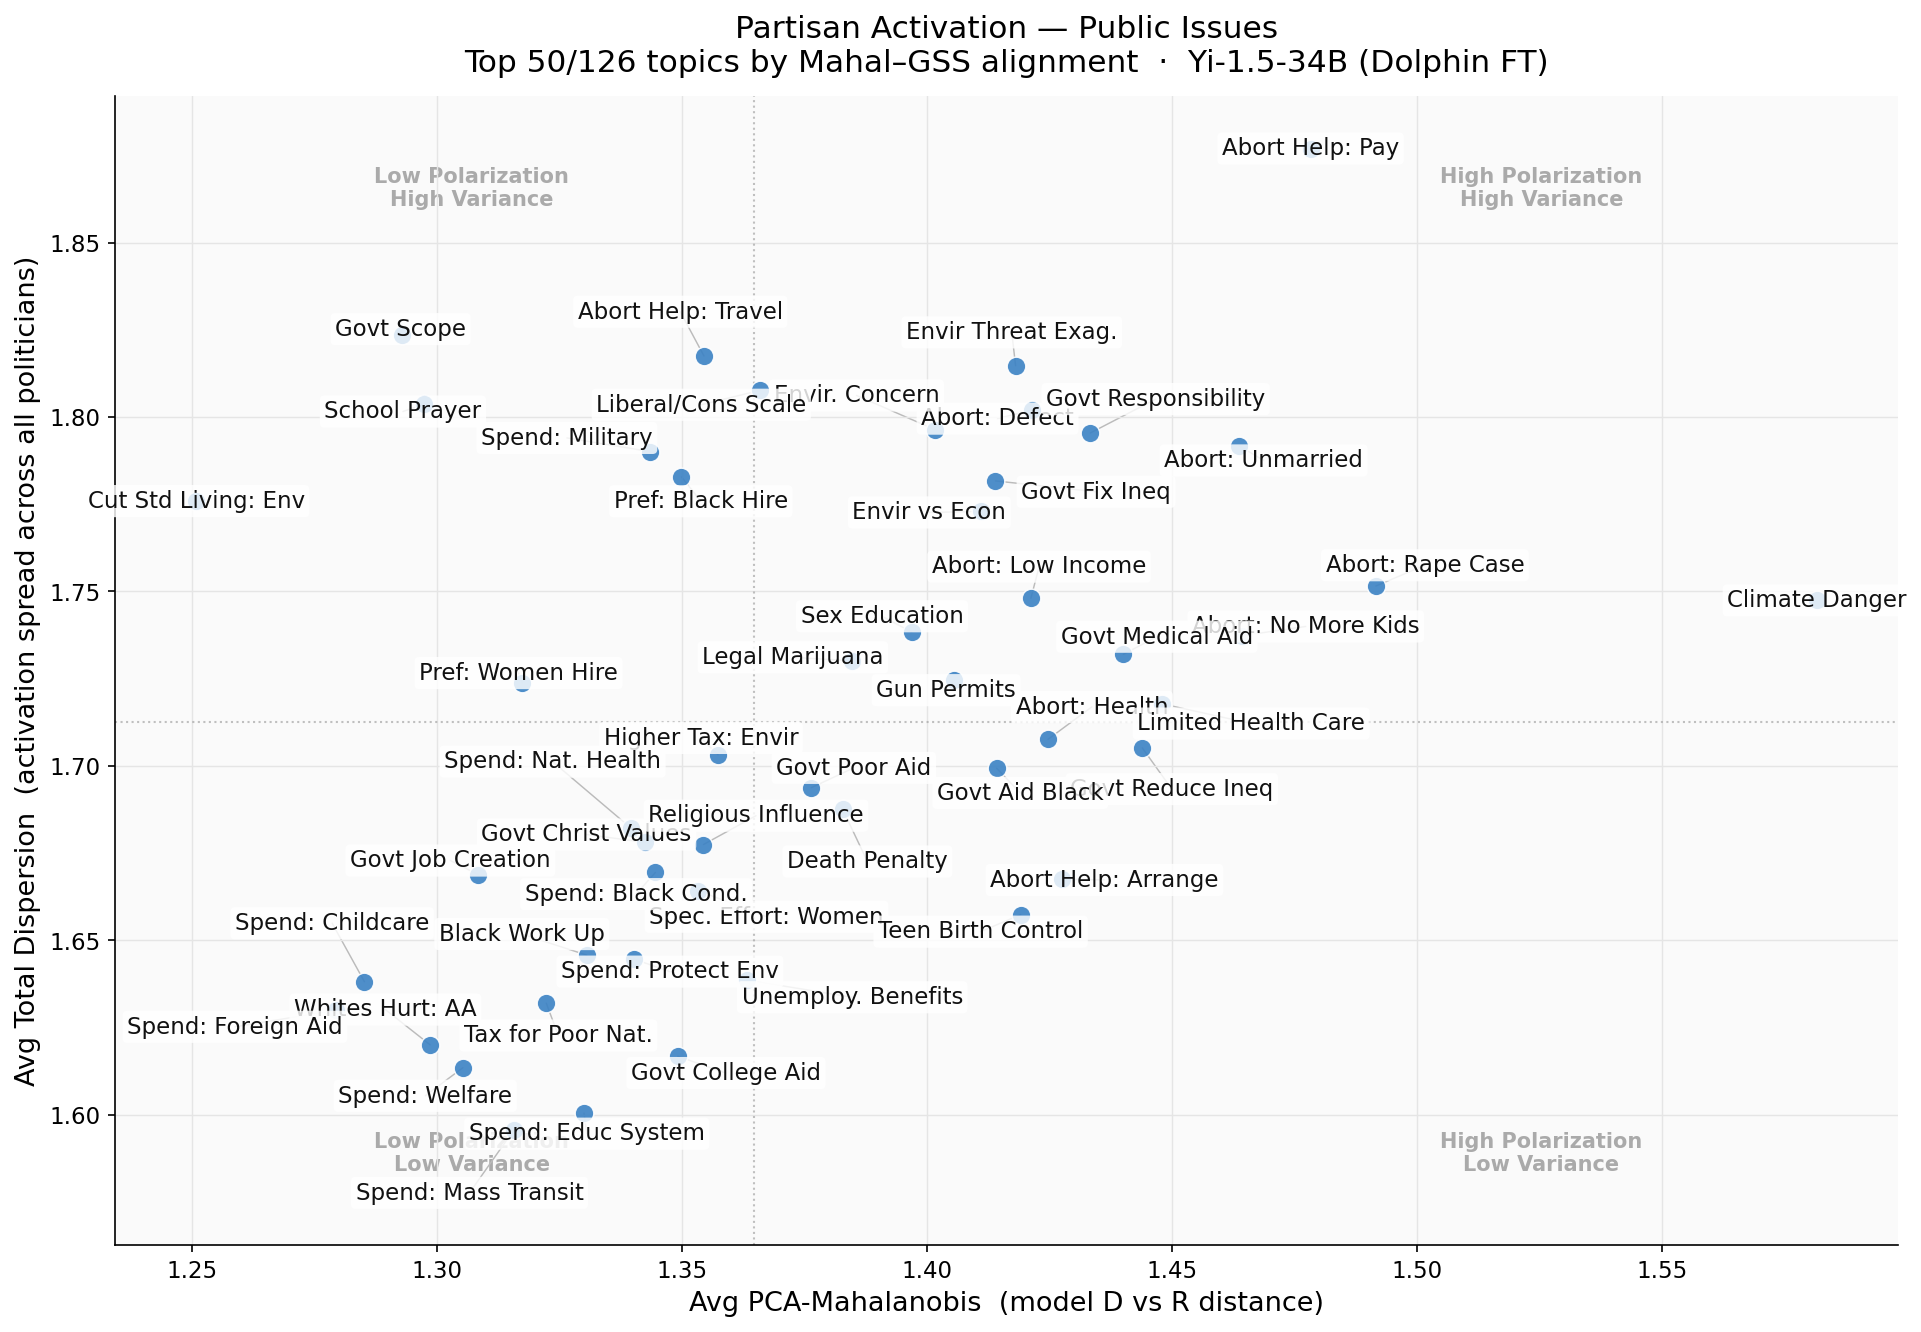
\includegraphics[width=\textwidth]{partisan_public_scatter.png}
\caption{Partisan activation geometry for \textbf{public issues} under dolphin-34B (stance). Each point is one of the top-50 topics (ranked by joint Mahal--GSS alignment). $x$-axis: mean PCA-Mahalanobis D--R distance; $y$-axis: mean total activation dispersion. Dotted lines mark axis medians.}
\label{fig:partisan_public}
\end{figure}

\begin{figure}[ht]
\centering
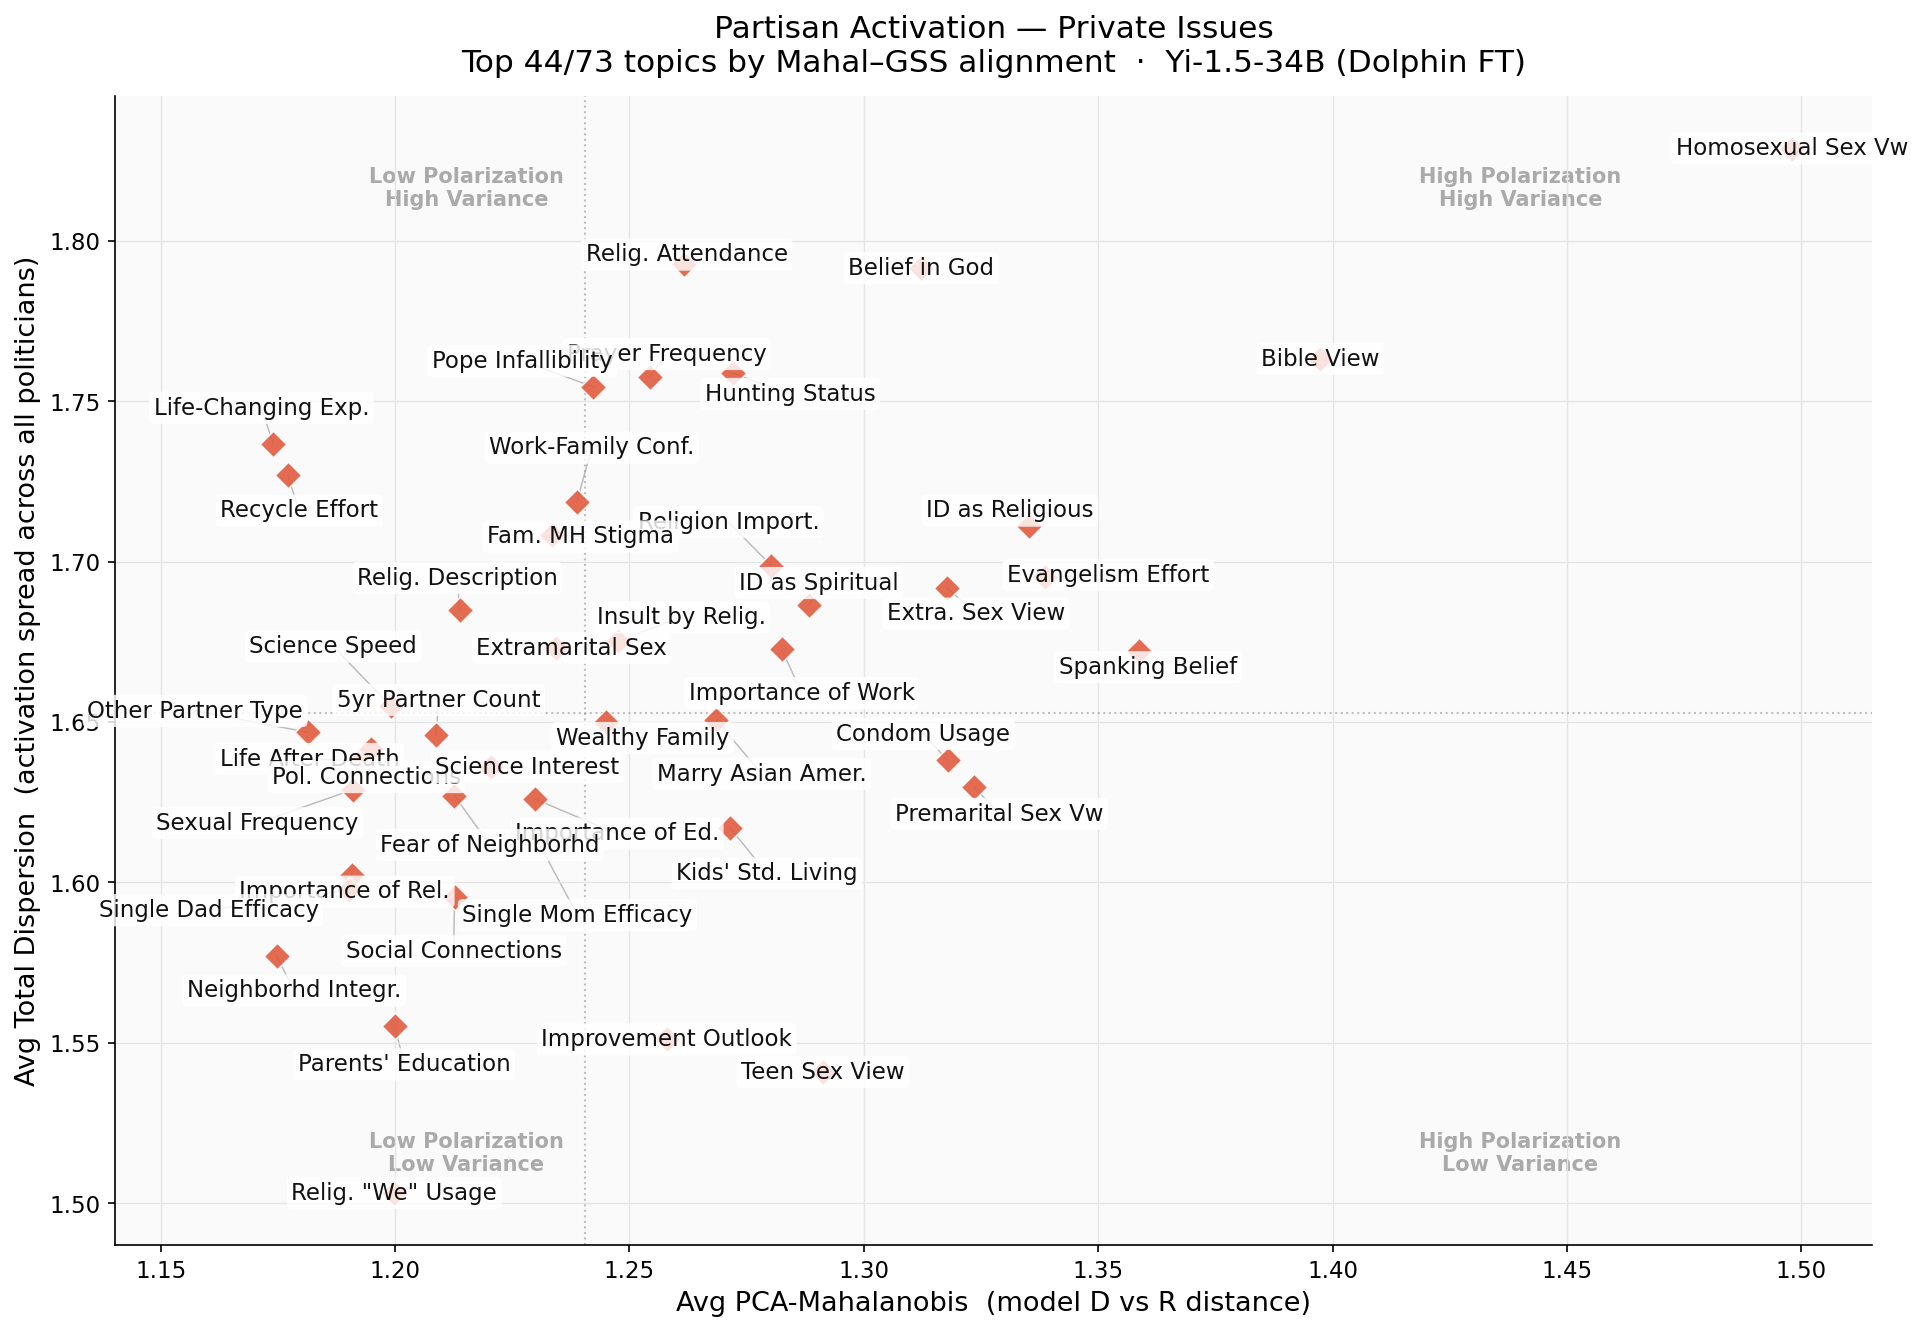
\includegraphics[width=\textwidth]{partisan_private_scatter.png}
\caption{Partisan activation geometry for \textbf{private-life issues} under dolphin-34B (stance). Top-44 topics by joint Mahal--GSS alignment. Axes and quadrant lines as in Figure~\ref{fig:partisan_public}.}
\label{fig:partisan_private}
\end{figure}

\end{document}
